% Give an overview of PUF devices

\chapter{Physically Unclonable Functions}
\label{chapter:pufoverview}
It is desirable for a user to be sure that the device that he is using is authentic. However, due to the sophistication
of forgeries or possible communication tampering, a user might be suspicious that the system is the system it claims
to be. A device called a Physically Unclonable Function, or PUF, is a technology that remedies this problem.

A PUF device provides a unique challenge-response capability. That is, when two PUFS are provided the identical
challenge, they will each produce unique responses. In this way, a PUF, and the system it contains, 
can be identified by the response value it generates to a specific challenge. A more formalized definition of
this relationship is given below.

\begin{align*}
PUF_1(C) = R_1\\
PUF_2(C) = R_2\\
R_1 \neq R_2
\end{align*}



\section{Types of PUFs}
A PUF device provides this sort of relationship by leveraging the physical properties
of the materials in which it is instantiated. There are several different ways of doing
this, from measuring the distortions of reflected light to leveraging the
manufacturing inconsistencies from one chip to another.

The Ring Oscillator PUF is presented first and in somewhat greater detail than
other types of PUF since this is the type of PUF that the author worked with primarily.
As such, it was incorporated in many of the different applications presented later in
Chapter ~\ref{chapter:applications}.

\subsection{Ring Oscillator PUF}
A Ring Oscillator PUF is a PUF design that utilizes a circuit called a Ring 
Oscillator (RO). An RO is an odd number of inverter gates tied together. Because
there are an odd number of gates, this will produce a continuously changing,
or oscillating, signal. 

\begin{figure}[h] % The h specifies to place the figure 'here' as in, inline with the source code
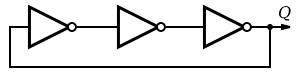
\includegraphics[]{images/ro.png}
\caption{A 3 gate Ring Oscillator}
\label{fig:ro}
\end{figure}

Depending on the number of inverter gates being used
as well as the propogation delay of every indiviudal inverter, the output
frequency of one RO may be different from another RO. In Figure ~\ref{fig:ro},
this output signal corresponds to the signal marked $Q$.

When used as part of a PUF, the unique behavior of an RO will be examined.
Consider again the 3 stage RO as shown in Figure ~\ref{fig:ro}. All three
inverter gates are assumed to have the same propogation delay and the
interconnecting wires are assumed to impose a neglible delay. However, in
an actual instationtion of an RO, these assumptions are invalid. All three inverters
should have the same propogation delay, but, due to uncontrollable manufacturing
inconsistencies and tolerances, they do not. In a similar vein, the interconnecting
wires will also impose a non-zero delay time in signal propogation. Both of these
factors will combine so that even if two ROs are produced on the same 
manufacturing line, they will generate a slightly different output frequency.

The slightly different output frequenices of two ring oscillators forms the basis
of randomness for the Ring Oscillator PUF. Because the output frequencies of the
ROs cannot be predicted, their actual frequency at runtime gives a way to uniquely
identify the individual PUF that contains them. In Figure ~\ref{fig:ropuf}, a more
detailed diagram of a PUF based off of ring oscillators is presented.

\begin{figure}[h]
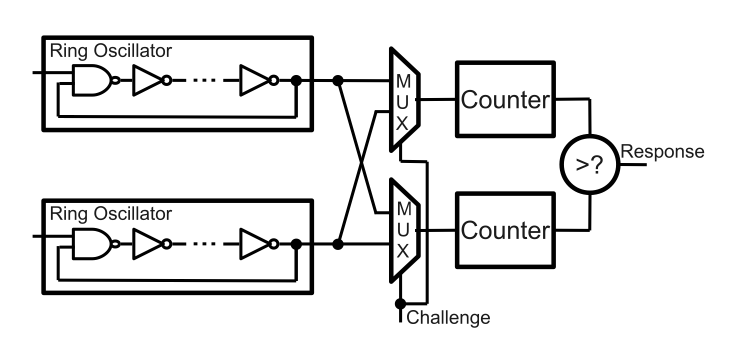
\includegraphics[width=500px]{images/ropuf.png}
\caption{A Basic Ring Oscillator Based PUF}
\label{fig:ropuf}
\end{figure}

As can be seen in Figure ~\ref{fig:ropuf}, the output of two ring oscillators is
fed into two multiplexers. Based on the challenge value, the multiplexers select
one of the output values and feed those into a counter. The counters measure the amount
of oscillations that occur over a given time period. At the end of the time period,
if the top counter has more oscillations, a 0 is recorded as the response, otherwise
a 1 is recorded as the response.

While the diagram only displays two ring oscillators and only 1 bit of challenge and
response, this diagram can be extrapolated to form arbitrarily large PUFs. Trivially,
the design can simply be copied so that an N-bit PUF requires 2N ring oscillators,
however, there are alternative methods that require a lesser amount of ring oscillators,
which in turn requires less space on a chip, which is desirable.

It is important to note that this PUF is not concerned with the absolute number of oscillations
of ring oscillators, but rather, with the \emph{relative} number of oscillations between
the two ring oscillators. This is because the counters are compared to each other, rather than
some absolute constant. This provides the benefit that if the entire circuit is heated or cooled,
which will in turn affect operating frequency, the PUF will still produce the same response, since
both oscillators were effected in the same way.

\subsection{Butterfly PUF}

\begin{figure}[h]
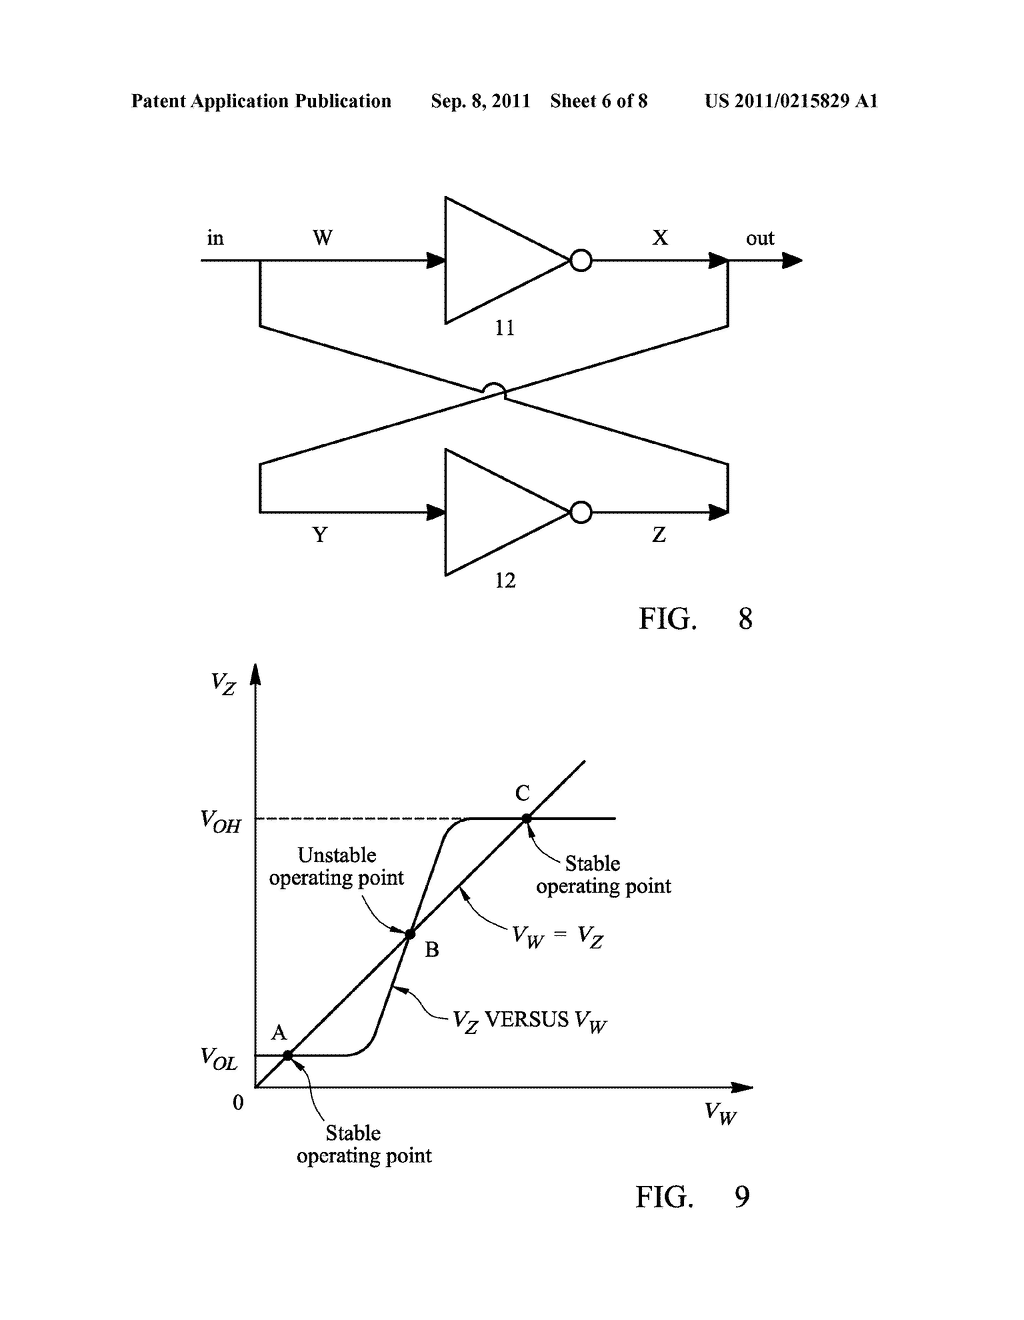
\includegraphics[width=500px]{images/butterflypuf.png}
\end{figure}

~\cite{butterflypuf}
\subsection{Optical PUF}

\subsection{Coating PUF}





\section{Vulnerabilities}
% Differential power analysis (security engineering, chapter 15)

% Tampering

\section{Comparison to Alternatives}

\subsection{Trusted Platform Module}

\subsection{Radio Frequency Identification Tags}

